\documentclass[preprint,12pt, authoryear, review]{elsarticle}
\usepackage[american]{babel}
\usepackage{lineno, csquotes, tipa, amsmath, caption, afterpage, booktabs}
\usepackage{hyperref}
\modulolinenumbers[5]

\journal{Neuropsychologia}


\begin{document}
	
	\begin{frontmatter}

%\title{Elsevier \LaTeX\ template\tnoteref{mytitlenote}}
%\tnotetext[mytitlenote]{Fully documented templates are available in the elsarticle package on \href{http://www.ctan.org/tex-archive/macros/latex/contrib/elsarticle}{CTAN}.}

	\title{Differential patterns of brain activity are correlated with sensitivity to morphological structure}

	%%% Group authors per affiliation:
	%\author{Elsevier\fnref{myfootnote}}
	%\address{Radarweg 29, Amsterdam}
	%\fntext[myfootnote]{Since 1880.}

	%	% Author list with affiliations and footnotes
	\author[pc]{Joanna Morris\corref{cor1}}
	\author[usc]{Emma Kealey\fnref{fn-pc}}
	\author[columbia]{Tess Rooney\fnref{fn-pc}\fnref{equal}}
	\author[brown]{Joemari Pulido\fnref{fn-pc}\fnref{equal}}
	\author[pc]{Natalia Alzate\fnref{equal}}
	\author[pc]{Ethan Moore\fnref{equal}}
	\author[pc]{Crismar Ramos-Marte\fnref{equal}}
	\author[ohsu]{Frankie Greene\fnref{fn-hc}}
	
	% Affiliation blocks
	\address[pc]{Department of Psychology, Providence College, Providence, RI, USA}
	\address[usc]{Department of Linguistics, University of Southern California, Los Angeles, CA, USA}
	\address[columbia]{Columbia University School of Nursing, New York, NY, USA}
	\address[brown]{Department of Cognitive, Linguistic \& Psychological Sciences, Brown University, Providence, RI, USA}
	\address[ohsu]{Oregon Health \& Science University and Portland State University School of Public Health, Portland, OR, USA}
	
	% Footnotes
	\cortext[cor1]{Corresponding author: Joanna Morris, jmorris6@providence.edu}
	\fntext[fn-pc]{Work conducted while affiliated with the Department of Psychology, Providence College, Providence, RI, USA}
	\fntext[fn-hc]{Work conducted while affiliated with the School of Cognitive Science, Hampshire College, Amherst, MA, USA}
	\fntext[equal]{These authors contributed equally to this work.}


	\begin{abstract}
	Skilled reading requires us to rapidly retrieve a word's meaning from memory based on a brief exposure to a sequence of arbitrary, abstract visual symbols. Within the lexicon, the mapping from form to meaning takes place at the level of morphology, and rapid semantic retrieval is facilitated by lexical representations that are precise, specific, redundant and flexible. Given that both lexical quality and sensitivity to morphological structure are key components of reading success, can we identify patterns of brain activity that reflect individual differences in these characteristics? To answer this question, we collected event-related potential and response time data from participants as they performed a lexical decision task designed to examine the effects of base frequency and morphological family size on processing both words and non-words. These data allowed us to determine individual differences in sensitivity to morphological structure. We also quantified individual differences in lexical quality (LQ) via estimates of vocabulary size and spelling performance, both of which are correlated with the precision and stability of lexical representations. We found differences between high LQ and low LQ participants in the N250 ERP component which has been hypothesised to reflect the processing sub-lexical orthographic units as well as in the N400. These findings suggest that individual differences in lexical quality and sensitivity to morphological structure are reflected in distinct patterns of brain activity, and opens the avenue for further work to investigate the perceptual and cognitive processes that underlie these differences.
	\end{abstract}
	
	
	%%Each keyword shall be separated by a \sep command. msc classifications shall be provided in the keyword  environment with the commands \MSC. \MSC accepts an optional argument to accommodate future revisions. eg., \MSC[2008]. The default is 2000.
	
	\begin{keyword}
	 morphology\sep event-related potentials\sep visual statistical learning \sep individual differences
	\end{keyword}

\end{frontmatter}

\linenumbers
\section{Introduction}

Reading is often defined as “the process of gaining meaning from print” \citep[][p.~34]{raynerHowPsychologicalScience2001}. Because words are the primary carriers of meaning, learning to recognize and decode them is central to becoming a fluent reader \citep[e.g.,][]{castlesEndingReadingWars2018}. While comprehension extends beyond single-word recognition to include inference, integration, and discourse-level processing, the efficiency with which readers access word meanings remains a cornerstone of skilled reading.

\subsection{Orthography, Morphology, and the Structure of English}

All writing systems map visual symbols onto units of spoken language, but they differ in which linguistic unit is targeted. Alphabetic scripts map letters to phonemes, syllabaries to syllables, and logographic systems to morphemes or words.\footnote{Although Chinese is often labeled logographic, its characters are better described as morpho-syllabic \citep{raynerHowPsychologicalScience2001}.} These mappings have profound consequences for how reading is acquired and processed. 

In alphabetic systems such as English, learning to read requires establishing mappings between graphemes and phonemes. The ease of this process depends on the language’s \textit{orthographic depth}—the regularity of the letter–sound correspondences. English is a deep orthography, with context-sensitive grapheme–phoneme mappings that vary by position and neighboring letters. However, English preserves regularities at higher representational levels: orthographic rimes (e.g., \textit{cat}, \textit{hat}, \textit{mat}) and morphemes (e.g., \textit{heal}–\textit{health}, \textit{help}–\textit{helpless}). This trade-off reflects a prioritization of morphological transparency over phonological consistency \citep{zieglerReadingAcquisitionDevelopmental2005, rastlePlaceMorphologyLearning2019}. 

Thus, skilled reading in English requires a flexible system that coordinates mappings from print to sound and to meaning across multiple linguistic units—phonemes, rimes, and morphemes alike. Awareness of all three units contributes to reading development \citep{mahonyReadingAbilitySensitivity2000}. Because many of these regularities are not taught explicitly, readers must infer them implicitly through \textit{statistical learning} (SL)—the domain-general ability to extract recurring patterns from experience. SL enables readers to internalize probabilistic associations among letters, sounds, and morphemes, forming the foundation of what we refer to as \textit{orthographic sensitivity}: the ability to detect and use structure in letter strings. This sensitivity develops gradually over the school years \citep{treimanSpellingStatisticalLearning2006}, varies substantially across individuals \citep{arciuliStatisticalLearningRelated2012}, and is a key determinant of reading fluency.

\subsection{Lexical Quality and the Precision of Word Representations}

To read fluently, readers must develop precise and well-integrated lexical representations. According to the \textit{Lexical Quality Hypothesis} \citep{perfettiLexicalQualityHypothesis2002, perfettiReadingAbilityLexical2007, perfettiLexicalQualityRevisited2017}, lexical quality reflects how completely a word’s orthographic, phonological, and semantic constituents are specified and interconnected. High-quality representations enable rapid, automatic activation of a word’s sound and meaning from its visual form, while low-quality representations are partial or underspecified and therefore slower and less reliable.

Individual variability in reading and spelling skill can be viewed as reflecting differences in lexical quality \citep{andrewsLexicalExpertiseReading2009, andrewsLexicalPrecisionSkilled2010, andrewsIndividualDifferencesSkilled2012}. Readers with more precise orthographic representations identify words quickly and resist interference from similar-looking forms, as demonstrated in masked form priming studies \citep{forsterRepetitionPrimingFrequency1984, andrewsLexicalPrecisionSkilled2010}. Conversely, readers who rely on coarse visual patterns or contextual guessing may read fluently but spell poorly, indicating less precise lexical representations \citep{frithSurfaceDevelopmentalDyslexia2017}. Such differences in lexical precision are likely rooted in the efficiency of statistical learning and sensitivity to orthographic regularities \citep{sharePhonologicalRecodingSelfteaching1995}.

\subsection{Individual Differences in Complex Word Recognition}

Traditional models of word recognition often assume a uniform cognitive architecture across skilled readers \citep{cronbachTwoDisciplinesScientific1957}. Yet evidence increasingly suggests that readers differ systematically in how they process morphological structure. Morphological priming studies show that complex words facilitate recognition of their stems, even when the prime–target pair is semantically opaque (e.g., \textit{corner–corn}) \citep{rastleBrothMyBrother2004, rastleMorphologicalDecompositionBased2008}. These findings imply that readers decompose complex words into sublexical morphemic units based on orthographic cues—a process known as \textit{morpho-orthographic decomposition}. 

However, meta-analytic work indicates that semantic transparency modulates these effects \citep{feldmanEarlyMorphologicalProcessing2009}, challenging purely form-driven accounts. Models grounded in statistical learning and distributed representations \citep{plautAreNonsemanticMorphological2000, baayenAmorphousModelMorphological2011} explain these discrepancies by positing that morphological structure emerges through learned correlations between orthography and meaning, yielding graded transparency effects. 

Crucially, \citet{andrewsMorphologicalPrimingStronger2013} showed that these competing results can be reconciled by considering \textit{individual differences}. Readers with stronger spelling than vocabulary skills—indicative of high orthographic precision—exhibited robust priming even for opaque pairs, suggesting an early reliance on form-based segmentation. Readers with stronger vocabulary than spelling skills—reflecting greater semantic sensitivity—showed priming only for transparent pairs, indicating that their morphological processing was constrained by meaning. These distinct “orthographic” and “semantic” profiles suggest two complementary routes to morphological processing: one driven by form-based decomposition and one guided by lexical-semantic integration.

\subsection{Frequency, Family Size, and Morphological Connectivity}

Morphologically complex words vary in how strongly their components are represented and connected in the lexicon. Three frequency-based measures are especially informative: \textit{surface frequency} (the occurrence of the whole word), \textit{base frequency} (the summed frequency of its stem across contexts), and \textit{morphological family size} (the number of derivationally related forms). High base frequency and large family size facilitate recognition \citep{taftRecognitionAffixedWords1979, schreuderMorphologicalFamilySize1997}, but they may reflect different underlying processes. Base frequency effects may arise from stronger stem representations, while family size effects capture semantic network connectivity among related words \citep{vannestCoActivationMorphologicalFamilies2011}. 

Both measures index morphological familiarity but at different levels—form versus meaning—and thus provide ideal test cases for probing whether readers rely more on orthographic or semantic cues during complex word recognition. The current study examines these effects not only in real words but also in morphologically structured nonwords, where semantic support is absent, allowing the role of form-level processing to be isolated.

\subsection{The Present Study}

The present experiment tested how individual differences in reading skill shape sensitivity to morphological structure during visual word recognition. Participants completed a lexical decision task while their EEG was recorded, allowing us to measure both behavioral and neural correlates of morphological processing. The stimuli included both words and morphologically structured nonwords (e.g., \textit{gasful} vs.~\textit{gasfil}), which were matched in surface form but differed in morphological plausibility. Morphological variables (\textit{Base Frequency}, \textit{Family Size}, and \textit{Morphological Complexity}) were manipulated orthogonally, and participants were grouped by either \textit{Orthographic Sensitivity} (indexed by spelling ability) or \textit{Language Proficiency} (indexed by vocabulary knowledge).

Based on prior research and on the distinction between form-based and meaning-based reading profiles, we predicted a functional dissociation between these individual-difference measures. Specifically, we expected Orthographic Sensitivity to modulate early form-based processing indexed by the \textit{N250}, reflecting efficient morpho-orthographic decomposition, whereas Language Proficiency would primarily modulate later, meaning-based integration indexed by the \textit{N400}. In behavioral terms, we expected Orthographic Sensitivity to influence overall response speed, while Language Proficiency would exert subtler effects visible primarily in neural indices of semantic integration. By examining both words and nonwords, we aimed to reveal how these two dimensions of reading skill—form decoding and semantic proficiency—jointly shape the time course of morphological processing in skilled readers.

\subsection{Conceptual Framework: A Dual-Pathway Model of Skilled Reading}

The present design is guided by a dual-pathway view of skilled reading in which orthographic and semantic expertise jointly determine how morphological information is processed. \textit{Orthographic Sensitivity} governs the efficiency of early form-based decoding—how rapidly and accurately readers parse letter strings into familiar sublexical units such as morphemes and affixes. This pathway supports automatic, bottom-up segmentation and is reflected behaviorally in overall response speed and neurally in early components such as the \textit{N250}. In contrast, \textit{Language Proficiency} governs later, top-down integration of meaning, guiding how morphological and semantic information are combined to form coherent lexical representations. This semantic pathway is indexed by modulations of the \textit{N400}, reflecting depth of processing and flexibility in meaning construction. 

According to this framework, skilled reading depends on the coordination of these two pathways: rapid morpho-orthographic decoding provides access to candidate word forms, while language proficiency determines how deeply those forms are interpreted and integrated. Readers with high orthographic sensitivity should thus show faster and more efficient early processing, whereas those with high language proficiency should show more differentiated neural responses to semantic and morphological relationships. The present study tests these predictions by examining how individual differences along both dimensions shape behavioral and electrophysiological responses to morphologically structured stimuli.


\begin{figure}[htbp]
	\centering
	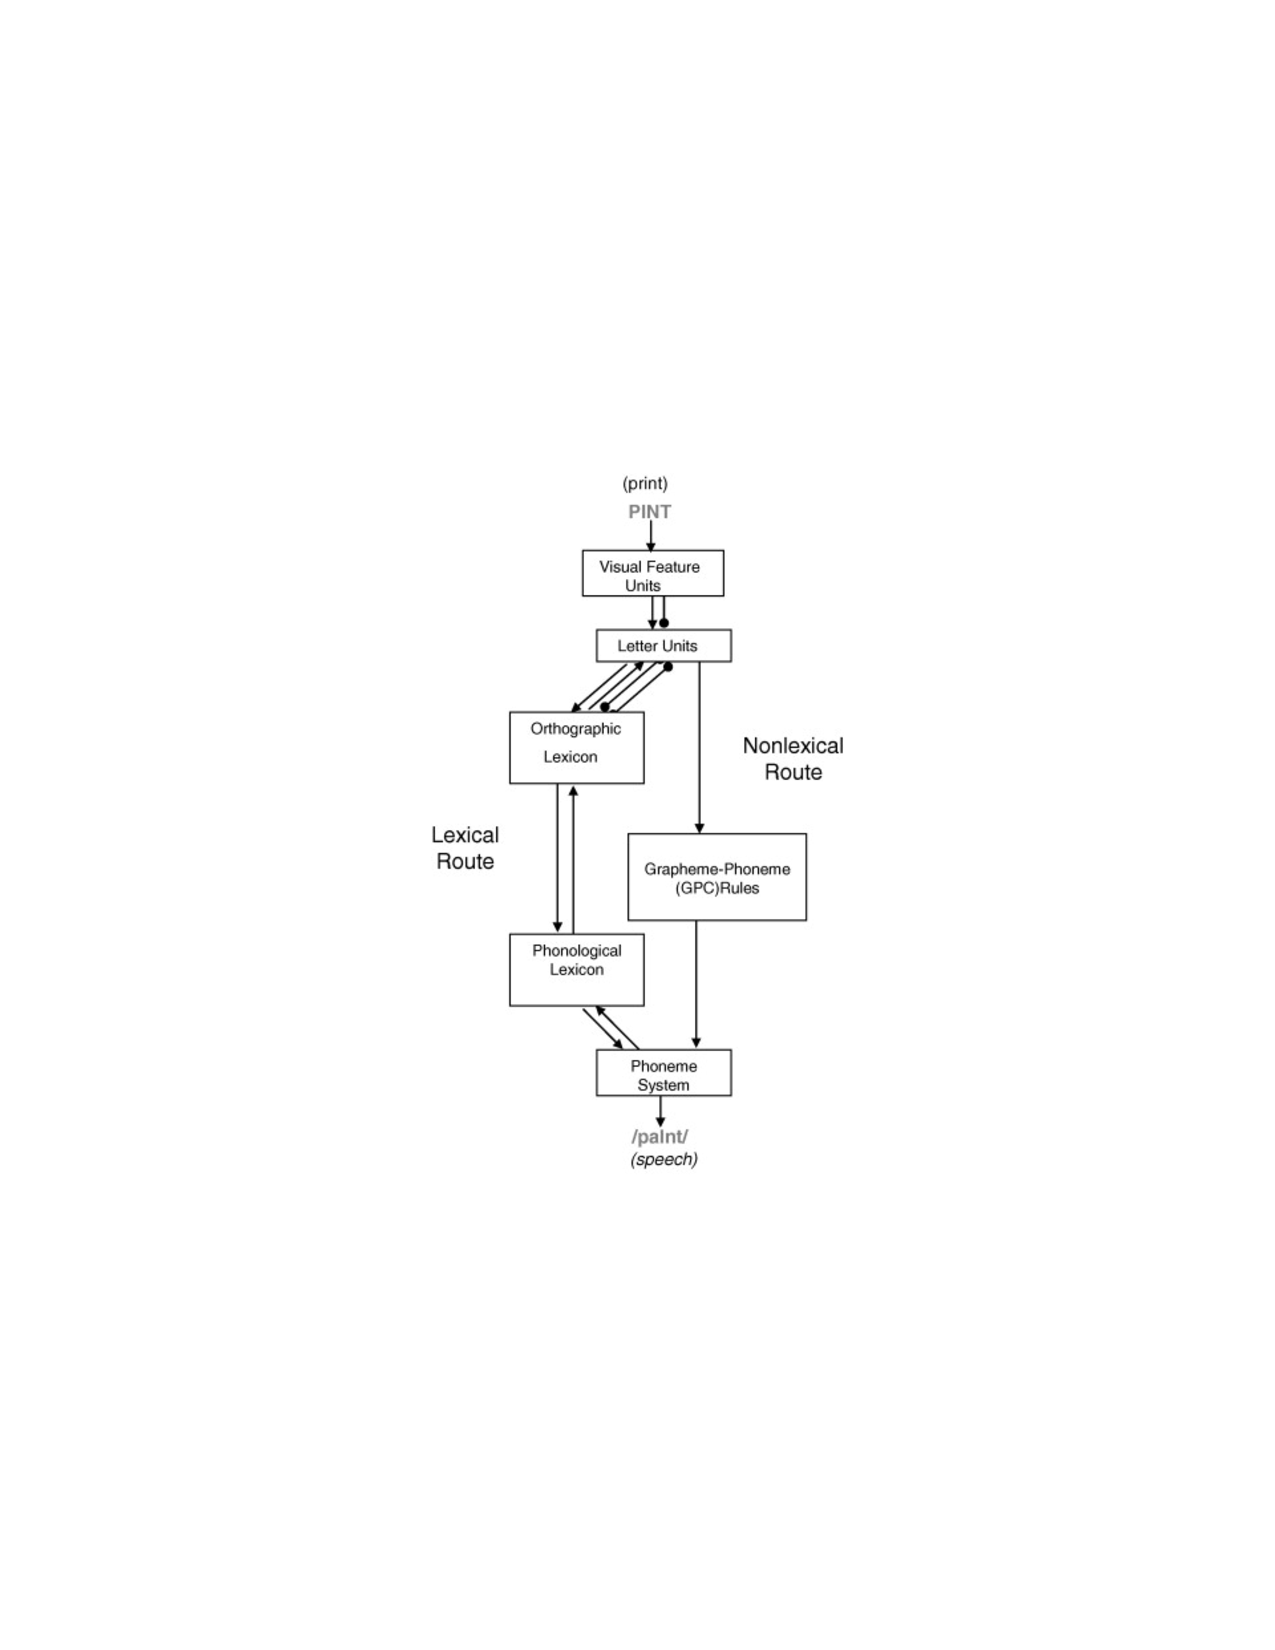
\includegraphics[width=.85\textwidth]{dual_pathway_model.pdf}
	\caption{\textbf{Dual-pathway model of morphological processing in skilled reading.} 
		The model proposes two partially independent but interacting routes that jointly support morphological processing during visual word recognition. 
		The \textit{form-decoding pathway}, driven by \textit{Orthographic Sensitivity}, operates early and bottom-up, supporting rapid parsing of letter strings into familiar sublexical units such as stems and affixes. This pathway is associated with faster reaction times and modulations of the \textit{N250} component, reflecting morpho-orthographic decomposition. 
		The \textit{semantic-integration pathway}, governed by \textit{Language Proficiency}, operates later and top-down, supporting the integration of morphological, lexical, and contextual information to derive meaning. This pathway is indexed by the \textit{N400} component, reflecting the depth and flexibility of semantic processing. 
		Efficient reading depends on the coordination of both pathways: form-level decoding provides rapid access to candidate lexical representations, while semantic proficiency determines how deeply those representations are interpreted and integrated.}
	\label{fig:dual_pathway_model}
\end{figure}


\section{Methods}

\subsection{Individual Differences and Grouping Variables}

To quantify individual differences in linguistic experience and orthographic knowledge, participants completed three standardized measures: a vocabulary test, a spelling test, and the Author Recognition Test (ART; Stanovich \& West, 1989). Scores on these measures were moderately correlated (\textit{r}s = .29–.51, all $p < .02$), indicating partially overlapping but distinct sources of variance in lexical experience.

A principal components analysis (PCA) was conducted on standardized (z-scored) vocabulary, spelling, and ART scores. Two components had eigenvalues greater than~1, jointly accounting for 83.5\% of the total variance (58.0\% for Dimension~1 and 25.5\% for Dimension~2). Component loadings (Table~\ref{tab:pca_loadings}) showed that Dimension~1 loaded most strongly on vocabulary and print exposure (ART), whereas Dimension~2 loaded most strongly on spelling accuracy:

\begin{itemize}
	\item[-] \textit{Dimension~1 (Language Proficiency)}: vocabulary (.82), ART (.81), spelling (.65)
	\item[-] \textit{Dimension~2 (Orthographic Sensitivity)}: spelling (.76), vocabulary ($-.29$), ART ($-.32$)
\end{itemize}

These results indicate that the first component captures general language proficiency—encompassing vocabulary knowledge and print exposure—while the second component reflects sensitivity to orthographic form. The two components were statistically independent ($r \approx 0$), supporting their interpretation as orthogonal individual-difference dimensions.

Participants were classified as \textit{High} or \textit{Low} on each component based on whether their standardized PCA score was above or below zero. Following this procedure, two independent grouping variables were derived: (1) \textit{Language Proficiency} (High vs.\ Low) and (2) \textit{Orthographic Sensitivity} (High vs.\ Low). All behavioral and ERP analyses were conducted twice—once grouping participants by Orthographic Sensitivity and once by Language Proficiency—using the same underlying dataset. This approach allows separate examination of whether morphological and lexical effects are modulated by spelling-based versus language-experience–based proficiency.

\begin{table}[ht]
	\centering
	\caption{PCA loadings and variance explained for the three lexical-experience measures.}
	\label{tab:pca_loadings}
	\begin{tabular}{lcc}
		\toprule
		\textbf{Measure} & \textbf{Dimension~1 (Language Proficiency)} & \textbf{Dimension~2 (Orthographic Sensitivity)} \\
		\midrule
		Vocabulary (z\_vcb) & 0.82 & $-0.29$ \\
		Spelling (z\_spl) & 0.65 & 0.76 \\
		Author Recognition Test (z\_art) & 0.81 & $-0.32$ \\
		\midrule
		\textit{Eigenvalue} & 1.74 & 0.76 \\
		\textit{Variance explained (\%)} & 58.0 & 25.5 \\
		\bottomrule
	\end{tabular}
\end{table}

\subsection{Statistical Analyses}

Analyses were conducted separately for three dependent measures: (1) response times (RTs) for correct lexical decisions, (2) mean N250 amplitudes, and (3) mean N400 amplitudes. All models were implemented in \textbf{R} (version~4.x) using the \texttt{afex}, \texttt{lme4}, and \texttt{emmeans} packages.
	
\paragraph{Reaction Time Analyses}

RTs for correct word trials were analyzed using linear mixed-effects models implemented in \texttt{afex::mixed}, employing the Satterthwaite (S) method for denominator degrees of freedom. Fixed effects included base frequency (“high” vs. “low”), morphological family size (“large” vs. “small”), and a between-subjects factor indexing reading ability, either orthographic sensitivity or language proficiency (median split). Each model was run twice, once for each grouping variable. The final model included by-subject random slopes for base frequency and morphological family size and took the form:

\begin{quote}
	{\scriptsize
		\texttt{ResponseTime ~ Base Frequency * Family Size * Sensitivity + (1 + Base Frequency + Family Size | SubjID) + (1 | ItemID)}
	}
\end{quote}

Random intercepts for subjects and lexical items, as well as by-subject random slopes, were included to account for individual and item-level variability. Likelihood-ratio tests (\texttt{ranova}) confirmed that both random effects significantly improved model fit ($\chi^2 > 170$, $p < 2 \times 10^{-16}$).
Effect sizes were computed as $\eta_p^2$ using \texttt{effectsize::eta\_squared}, and model fit was summarized by marginal (fixed-effects) and conditional (fixed + random-effects) $R^2$ values obtained with \texttt{performance::r2}. RTs for non-word trials were analyzed separately because non-words varied by morphological complexity (“simple” vs. “complex”) and could be classified either by base frequency (“high” vs. “low”) or by family size (“large” vs. “small”), but not both simultaneously. Accordingly, two parallel models were run for each participant grouping variable (orthographic sensitivity and language proficiency), yielding four non-word RT analyses in total. These models followed the general form:

\begin{quote}
	{\scriptsize
		\texttt{ResponseTime ~ Complexity * Frequency or FamilySize * Sensitivity + (1 + Complexity | SubjID) + (1 | ItemID)}
	}
\end{quote}

\paragraph{ERP Analyses}

Mean ERP amplitudes were analyzed separately for the N250 (150–250~ms) and N400 (300–500~ms) time windows and for word and non-word datasets. For each combination of time window and lexicality, the same model structure was applied twice—once incorporating orthographic sensitivity and once language proficiency as the between-subjects factor—yielding parallel models for each ERP component and lexicality. Each model predicted mean amplitude as a function of sensitivity or proficiency, morphological complexity (for non-words only), and either family size or base Frequency, including all interactions.

Random effects included by-subject intercepts and slopes for within-subject factors and random intercepts for electrode site (\texttt{chlabel}) nested within subject. The general model form was:


	{\scriptsize \texttt{Amplitude ~ Sensitivity * Family Size * Complexity + (1 + Family Size + Complexity | SubjID) + (1 | SubjID:chlabel)}}


Degrees of freedom and $p$-values were computed using the Kenward–Roger approximation (\texttt{afex}). Significant interactions were followed up with estimated marginal means (EMMs) and pairwise contrasts (\texttt{emmeans}).

\paragraph{Statistical Justification}

Linear mixed-effects modeling was chosen because it allows simultaneous estimation of both subject- and item-level variability, providing a more generalizable assessment of fixed effects than traditional repeated-measures ANOVA (Baayen, Davidson, \& Bates, 2008; Barr et al., 2013). By including random intercepts for participants and lexical items, as well as by-subject random slopes for within-subject factors where appropriate, these models account for the hierarchical structure of the data and reduce the risk of inflated Type~I error due to nonindependent observations. The use of the Satterthwaite and Kenward–Roger approximations for denominator degrees of freedom yields valid inferential tests under realistic unbalanced designs common in EEG and psycholinguistic data.


\paragraph{Reporting Structure}

The results are presented in two parts. We first report the reaction time (RT) analyses, which assess behavioral sensitivity to morphological and lexical variables, followed by the ERP analyses, which examine how these effects unfold over time in the N250 and N400 components. Within each domain, analyses are reported separately for words and non-words and, in turn, for models incorporating orthographic sensitivity and general language proficiency as between-subject factors. These parallel analyses provide complementary perspectives on how reading skill modulates both behavioral and neural measures of morphological processing.


\section{Results}

We first report the reaction time (RT) analyses, which assess behavioral sensitivity to morphological and lexical variables, followed by the ERP analyses, which examine how these effects unfold over time in the N250 and N400 components. Within each domain, results are shown separately for words and non-words and for models incorporating orthographic sensitivity and general language proficiency as between-subject factors. These parallel analyses provide complementary perspectives on how reading skill modulates both behavioral and neural measures of morphological processing.

\subsection{Response Time Data with participants grouped by Orthographic Sensitivity}
		
	\subsubsection{Words} 
		
		We found a significant main effect of Base Frequency in that participants responded more quickly to words derived from high-frequency bases, ($M = 602$ ms, SE = 9.6) than to those from low-frequency bases ($M = 622$ ms, SE = 10.1), $F(1, 93.84) = 10.22$, $p = .002$, $\eta_p^2 = .10$—an average facilitation of about 20 ms. A separate main effect of Family Size was also observed,$ F(1, 92.69) = 9.12$, $p = .003$, $\eta_p^2 = .09$, reflecting faster responses to words from large morphological families ($M = 603$ ms, SE = 9.9) than to words from small families ($M = 622$ ms, SE = 9.9). These two effects were additive; the Base Frequency × Family Size interaction was not significant, $F(1, 93.09) = 1.1$, $p = .30$, $\eta_p^2 = .01$. Orthographic Sensitivity showed only a nonsignificant trend toward faster RTs for higher-sensitivity participants, $F(1, 64.87) = 3.84$, $p = .054,$ $\eta_p^2 = .06$. High-OS participants averaged 595 ms (SE = 12.5), whereas Low-OS participants averaged 630 ms (SE = 13.4). No higher-order interactions approached significance. 
			
		The model explained 36\% of the total variance when both fixed and random effects were included (Conditional $R^2 = .36$), while fixed effects alone accounted for about 3\% (Marginal $R^2 = .03$). These values are comparable to those obtained in the simpler random‐intercept model and are consistent with typical lexical‐decision data, in which between‐subject and item variability dominate.
		
	\subsubsection{Nonwords}
	
		Response times to nonwords were analyzed as a function of morphological complexity, item-level characteristics (family size or base frequency), and individual differences in sensitivity (orthographic or semantic). Separate models were fit for nonwords grouped by either family size or base frequency.
	
		\paragraph{Non-word Reaction Times (Orthographic Sensitivity × Base Frequency)}
	
		The model revealed significant main effects of Complexity, $F(1,62.46)=93.48$, $p<.001$, $\eta^2_p=.60$, Base Frequency, $F(1,91.60)=11.72$, $p<.001$, $\eta^2_p=.11$, and Orthographic Sensitivity, $F(1,63.49)=5.27$, $p=.025$, $\eta^2_p=.08$. The Complexity × Base Frequency interaction approached significance, $F(1,4492.31)=3.84$, $p=.050$, $\eta^2_p<.01$, whereas no other interactions were reliable ($p>.52$). The model explained 5\% of the fixed-effect variance ($R^2_{marginal}=.05$) and 46\% of the total variance including random effects ($R^2_{conditional}=.46$).
	
		Overall, responses to complex non-words (736 ms) were slower than to simple ones (701 ms), and high-frequency bases elicited slower responses (729 ms) than low-frequency bases (708 ms). Participants with high orthographic sensitivity responded more quickly (695 ms) than those with low sensitivity (743 ms). The marginal Complexity × Base Frequency interaction  reflected a slightly larger Complexity effect for high-frequency bases; however, the direction of the effect was consistent across frequency conditions, suggesting a broadly uniform influence of morphological complexity.


		\paragraph{Non-word Reaction Times (Orthographic Sensitivity $\times$ Family Size)}
	
		The model revealed significant main effects of Complexity, $F(1, 62.51) = 91.00$, $p < .001$, $\eta^2_p = .59$, and Orthographic Sensitivity, $F(1, 63.54) = 5.33$, $p = .024$, $\eta^2_p = .08$, but no main effect of Family Size, $F(1, 95.24) = 1.03$, $p = .313$, $\eta^2_p = .01$. No interactions were significant ($p > .34$). The model accounted for 4.5\% of the fixed-effect variance ($R^2_{\text{marginal}} = .045$) and 46\% of the total variance including random effects ($R^2_{\text{conditional}} = .461$). Likelihood-ratio tests indicated that inclusion of item-level random intercepts significantly improved model fit, $\chi^2(1) = 144.39$, $p < 2 \times 10^{-16}$, whereas random slopes for Complexity or Family Size did not ($p > .38$).
	
		Across conditions, responses to complex non-words (736 ms) were slower than to simple ones (701 ms), and participants with high orthographic sensitivity responded faster (695 ms) than those with low sensitivity (743 ms). Mean RTs did not differ reliably for large (722 ms) versus small (716 ms) morphological families, and none of the interactions involving family size approached significance.

		
	\subsubsection{Summary of Response Time Results (Orthographic Sensitivity)}
		
	Across both words and non-words, participants with high orthographic sensitivity consistently responded more quickly than those with low sensitivity, indicating that greater sensitivity to orthographic structure facilitated lexical decision performance. For word stimuli, response times were independently influenced by both Base Frequency and Family Size: words derived from high-frequency bases and from large morphological families were recognized more rapidly, and these effects were additive. For non-word stimuli, robust effects of Morphological Complexity were observed in both analyses, with slower responses to complex than to simple items. Non-word response times also showed a modest main effect of Orthographic Sensitivity but only limited effects of lexical variables: Base Frequency produced slower responses for high-frequency bases, and Family Size did not reliably influence responses. 
	
	Taken together, these results suggest that orthographic sensitivity modulates overall response speed, while item-level frequency and morphological structure have dissociable influences depending on lexical status—facilitatory for real words but minimal or inhibitory for novel, morphologically structured non-words.
		
	\begin{table}[ht]
		\centering
		\caption{Summary of Response Time Results by Orthographic Sensitivity}
		\begin{tabular}{lccccc}
			\toprule
			\textbf{Dataset} & \textbf{Factor} & \textbf{$F$ (df)} & \textbf{$p$} & \textbf{$\eta^2_p$} & \textbf{Direction of Effect} \\
			\midrule
			\textit{Words} & Base Frequency & $F(1, 93.84) = 10.22$ & .002 & .10 & high $<$ low (faster) \\
			& Family Size & $F(1, 92.69) = 9.12$ & .003 & .09 & large $<$ small (faster) \\
			& Orthographic Sensitivity & $F(1, 64.87) = 3.84$ & .054 & .06 & high $<$ low (trend) \\
			\midrule
			\textit{Non-words (Base Frequency)} & Morphological Complexity & $F(1, 62.46) = 93.48$ & $< .001$ & .60 & complex $>$ simple (slower) \\
			& Base Frequency & $F(1, 91.60) = 11.72$ & $< .001$ & .11 & high $>$ low (slower) \\
			& Orthographic Sensitivity & $F(1, 63.49) = 5.27$ & .025 & .08 & high $<$ low (faster) \\
			\midrule
			\textit{Non-words (Family Size)} & Morphological Complexity & $F(1, 62.51) = 91.00$ & $< .001$ & .59 & complex $>$ simple (slower) \\
			& Family Size & $F(1, 95.24) = 1.03$ & .313 & .01 & ns \\
			& Orthographic Sensitivity & $F(1, 63.54) = 5.33$ & .024 & .08 & high $<$ low (faster) \\
			\bottomrule
		\end{tabular}
	\end{table}

\subsection{Response Time Data with participants grouped by language proficiency}

	\subsubsection{Words (Language Proficiency × Family Size × Base Frequency) }
	
	We found significant main effects of Base Frequency, $F(1, 93.30) = 10.16$, $p = .002$, $\eta_p^2 = .10$, and Family Size, $F(1, 88.08) = 9.06$, $p = .003$, $\eta_p^2 = .09$, indicating that participants responded more quickly to words derived from high-frequency bases ($M = 601$ ms, $SE = 9.8$) than to those from low-frequency bases ($M = 621$ ms, $SE = 10.3$), and to words from large morphological families ($M = 602$ ms, $SE = 10.0$) than to those from small families ($M = 620$ ms, $SE = 10.1$). These two effects were additive; the Base Frequency × Family Size interaction was not significant, $F(1, 92.22) = 1.01$, $p = .32$, $\eta_p^2 = .01$. 
	
	Language Proficiency did not yield a main effect, $F(1, 64.88) = 0.00$, $p = .990$, $\eta_p^2 < .001$, nor did it interact with any of the item-level factors (all $p > .54$). Thus, differences in language proficiency did not modulate the pattern of item-level frequency effects in word recognition. 
	
	The model explained approximately 1.7\% of the variance attributable to fixed effects ($R^2_{\text{marginal}} = .017$), consistent with the dominance of subject- and item-level variability in lexical decision response times. Likelihood-ratio tests confirmed that random intercepts for both subjects and items improved model fit, $\chi^2 > 170$, $p < 2 \times 10^{-16}$, while inclusion of random slopes did not ($p > .41$).
	
	\subsubsection{Nonwords}
	
	Response times to nonwords were analyzed as a function of morphological complexity, item-level properties (Family Size or Base Frequency), and Language Proficiency. Separate models were fit for nonwords grouped by family size and by base frequency.
	
	\paragraph{Non-word Reaction Times (Language Proficiency × Family Size)}
	
	The model revealed a significant main effect of Complexity, $F(1, 62.65) = 88.28$, $p < .001$, $\eta_p^2 = .58$, but no main effects of Family Size, $F(1, 94.52) = 0.91$, $p = .344$, $\eta_p^2 = .01$, or Language Proficiency, $F(1, 63.40) = 0.00$, $p = .957$, $\eta_p^2 < .001$. The three-way interaction among Complexity, Family Size, and Language Proficiency was significant, $F(1, 4387.63) = 4.73$, $p = .030$, $\eta_p^2 = .001$, whereas all two-way interactions were nonsignificant ($p > .49$). The model accounted for 1.6\% of the variance explained by fixed effects ($R^2_{\text{marginal}} = .016$) and 46\% of the total variance ($R^2_{\text{conditional}} = .462$). 
	
	Across conditions, responses to complex nonwords ($M = 734$ ms, $SE = 11.5$) were slower than to simple ones ($M = 700$ ms, $SE = 11.3$). Mean RTs did not differ significantly between large-family ($M = 720$ ms) and small-family ($M = 714$ ms) nonwords, nor between high-proficiency ($M = 716$ ms) and low-proficiency ($M = 717$ ms) participants. Follow-up contrasts showed that for high-proficiency participants, the complexity effect was larger for large-family nonwords ($\approx 45$ ms) than for small-family nonwords ($\approx 27$ ms), whereas low-proficiency participants showed little or no difference. These results indicate that higher language proficiency magnified the processing cost of morphological complexity for nonwords derived from large morphological families, suggesting greater sensitivity to morphological structure among more proficient readers.
	
	\paragraph{Non-word Reaction Times (Language Proficiency × Base Frequency)}
	
	The model revealed significant main effects of Complexity, $F(1, 62.89) = 90.74$, $p < .001$, $\eta_p^2 = .59$, and Base Frequency, $F(1, 90.71) = 11.45$, $p = .001$, $\eta_p^2 = .11$. Neither Language Proficiency nor any of its interactions were significant ($p > .30$). A marginal Complexity × Base Frequency interaction, $F(1, 4491.15) = 3.56$, $p = .059$, $\eta_p^2 < .01$, reflected a slightly smaller complexity cost for nonwords derived from low-frequency bases.
	
	Overall, participants responded more slowly to complex nonwords ($M = 734$ ms, $SE = 11.4$) than to simple ones ($M = 699$ ms, $SE = 11.2$), and to high-frequency-base nonwords ($M = 727$ ms, $SE = 11.3$) than to low-frequency-base nonwords ($M = 707$ ms, $SE = 11.9$). The model explained 2.1\% of the fixed-effect variance ($R^2_{\text{marginal}} = .021$) and 46\% of the total variance ($R^2_{\text{conditional}} = .462$). The direction of effects was consistent across proficiency groups, indicating that differences in language proficiency did not modulate the influence of base frequency or morphological complexity on nonword decision latencies.
	
	\subsubsection{Summary of Response Time Results (Language Proficiency)}
	
	Across both words and nonwords, participants with high and low language proficiency showed comparable overall response times, indicating that general language proficiency did not exert a robust effect on lexical decision performance. For words, response times were independently influenced by Base Frequency and Family Size, with faster responses to words derived from high-frequency bases and from large morphological families. For nonwords, robust effects of Morphological Complexity were again observed, with slower responses to complex than to simple items. Only one interaction involving Language Proficiency reached significance: in the family-size model, high-proficiency participants showed a stronger complexity effect for large-family nonwords, suggesting that proficiency modulates sensitivity to morphological family cues when processing unfamiliar forms. 
	
	Together, these results suggest that while item-level lexical variables (Base Frequency, Family Size, and Complexity) robustly shape response times, individual differences in language proficiency exert subtler influences—detectable primarily in how morphological structure interacts with complexity in the processing of novel forms.
	
	\begin{table}[ht]
		\centering
		\caption{Summary of Response Time Results by Language Proficiency}
		\begin{tabular}{lccccc}
			\toprule
			\textbf{Dataset} & \textbf{Factor} & \textbf{$F$ (df)} & \textbf{$p$} & \textbf{$\eta^2_p$} & \textbf{Direction of Effect} \\
			\midrule
			\textit{Words} & Base Frequency & $F(1, 93.30) = 10.16$ & .002 & .10 & high $<$ low (faster) \\
			& Family Size & $F(1, 88.08) = 9.06$ & .003 & .09 & large $<$ small (faster) \\
			& Language Proficiency & $F(1, 64.88) = 0.00$ & .990 & <.001 & ns \\
			\midrule
			\textit{Non-words (Base Frequency)} & Morphological Complexity & $F(1, 62.89) = 90.74$ & $< .001$ & .59 & complex $>$ simple (slower) \\
			& Base Frequency & $F(1, 90.71) = 11.45$ & .001 & .11 & high $>$ low (slower) \\
			& Language Proficiency & $F(1, 63.36) = 0.00$ & .970 & <.001 & ns \\
			\midrule
			\textit{Non-words (Family Size)} & Morphological Complexity & $F(1, 62.65) = 88.28$ & $< .001$ & .58 & complex $>$ simple (slower) \\
			& Family Size & $F(1, 94.52) = 0.91$ & .344 & .01 & ns \\
			& Language Proficiency & $F(1, 63.40) = 0.00$ & .957 & <.001 & ns \\
			& Complexity × Family Size × Language Proficiency & $F(1, 4387.63) = 4.73$ & .030 & .001 & sig. three-way \\
			\bottomrule
		\end{tabular}
	\end{table}


\subsection{ERP data with participants grouped by langauge proficiency}

\subsubsection{N250 Component}

\paragraph{Words}

The mixed-effects model for word stimuli included fixed effects of Family Size, Base Frequency, and Language ProficiencySensitivity and their interactions, with random slopes for Family Size and Base Frequency by subject and random intercepts for electrode (nested within subject). The model revealed no significant main effects. However, two interactions were significant: Family Size × Base Frequency, $F(1, 1498) = 32.72$, $p < .001$, $\eta_p^2 = .02$, and a three-way Language Proficiency × Family Size × Base Frequency interaction, $F(1, 1498) = 16.96$, $p < .001$, $\eta_p^2 = .01$. Follow-up contrasts indicated that for large-family words, N250 amplitude was more negative when Base Frequency was high than when it was low ($p = .029$), whereas for small-family words, Base Frequency had little effect. When Base Frequency was low, small-family words elicited more negative amplitudes than large-family words ($p = .016$). This pattern was further modulated by Language Proficiency: the base-frequency effect differed sharply between large- and small-family words for high-sensitivity participants ($-1.19$ $\mu V$, $95\% \text{CI} [-1.52, -0.86]$, $p < .001$), but not for low-sensitivity participants ($p = .27$). Thus, high-semantic participants showed a clear reversal of the base-frequency effect across family sizes—large for high-frequency items, small for low-frequency—whereas low-semantic participants showed no reliable modulation.

\paragraph{Nonwords}

For nonword stimuli, the model included fixed effects of Family Size, Complexity, and Language Proficiency and their interactions. A significant three-way interaction emerged, $F(1, 1498) = 4.71$, $p = .030$, $\eta_p^2 = .003$. Examination of simple effects showed that for low-semantic participants, large-family complex nonwords elicited more negative N250 amplitudes than simple ones, whereas high-semantic participants showed minimal differences across complexity or family size. Thus, at the N250, low-proficiency readers demonstrated stronger morphological-complexity effects for large-family nonwords, while high-proficiency readers exhibited reduced or absent complexity modulation—suggesting that early morpho-orthographic parsing is more effortful for less semantically skilled participants.

\subsubsection{N400 Component}

\paragraph{Words}

For words, the model with Family Size, Base Frequency, and Language Proficiency as fixed effects revealed a robust Family Size × Base Frequency interaction, $F(1, 1498) = 64.68$, $p < .001$, $\eta_p^2 = .04$, which was further modulated by Language Proficiency, $F(1, 1498) = 12.12$, $p < .001$, $\eta_p^2 = .008$.
Pairwise comparisons showed that when Base Frequency was low, large-family words elicited less negative N400s than small-family words ($p = .002$), but when Base Frequency was high, the family-size difference disappeared. Conversely, for small-family words, high-frequency bases produced more negative N400s than low-frequency ones ($p = .0003$). This interaction pattern was strongest in high-semantic participants, for whom the base-frequency effect flipped direction between large- and small-family words ($\Delta \; \approx 1.48 \mu V$, $p < .0001$), and weaker but still significant in low-semantic participants ($\Delta \; \approx 0.58 \mu V$, $p = .002$). In sum, high-proficiency participants showed larger and more differentiated N400 frequency effects, indicating that they engage semantic networks more deeply during morphological access, whereas low-proficiency participants displayed a reduced, flattened version of this pattern.

\paragraph{Nonwords}

For nonwords, the model revealed main and interaction effects of Complexity, $F(1, 58) = 4.15$, $p = .046$, $\eta_p^2 = .07$, Family Size × Complexity, $F(1, 1498) = 8.08$, $p = .005$, $\eta_p^2 = .005$, and a strong three-way Language Proficiency × Family Size × Complexity interaction, $F(1, 1498) = 34.43$, $p < .001$, $\eta_p^2 = .02$.

Simple-effects tests showed opposite patterns across groups:
High-semantic participants exhibited a greater complexity effect for small-family nonwords than for large ones.
Low-semantic participants showed the reverse—stronger complexity effects for large-family nonwords and little effect for small ones.
This interaction suggests that high-proficiency readers use familiarity (family size) to neutralize morphological-complexity effects, while low-proficiency readers show amplified complexity responses when encountering familiar morphemic patterns, reflecting heavier reliance on semantic co-activation.

\subsubsection{Summary Across Components}

Across both ERP time windows, effects of language proficiency consistently interacted with morphological variables rather than producing direct amplitude shifts.
At the N250, high-proficiency readers displayed more efficient, selective early parsing, with diminished complexity effects, whereas low-proficiency readers showed enhanced sensitivity to morphological structure at this early stage.

At the N400, proficiency effects emerged more robustly: for words, high-proficiency participants exhibited stronger integration of Family Size and Base Frequency, while for nonwords, they suppressed complexity effects that remained pronounced in low-proficiency readers.
Together, these findings indicate that greater language proficiency modulates both early and late stages of morphological processing—attenuating morpho-orthographic demands (N250) and facilitating semantic integration (N400).

		
\section{Discussion}

The present study investigated how morphological and lexical factors influence visual word recognition and how these effects vary with individual differences in reading skill. By combining behavioral and electrophysiological measures, we sought to clarify when and how readers engage morphological structure during lexical access, and how this engagement depends on \textit{Orthographic Sensitivity} and \textit{Language Proficiency}. The findings converge on a view of morphological processing as an interactive, multi-stage system in which base-level familiarity and family-level connectivity make distinct contributions that are tuned by individual skill.

\subsection{Behavioral Patterns: Additive Facilitation for Words and Morphological Interference for Nonwords}

The reaction time (RT) results demonstrate that morphological and lexical variables exert reliable, dissociable influences on visual word recognition. For words, both \textit{Base Frequency} and \textit{Family Size} facilitated recognition independently, indicating that familiarity with the base morpheme and connectivity within the morphological family each promote faster lexical access. The additive nature of these effects implies that stem-level familiarity and family-level activation operate through partially distinct mechanisms that converge on a shared decision process. 

In contrast, \textit{nonwords} elicited the opposite pattern: morphologically complex pseudowords were rejected more slowly than unstructured controls, and higher base frequency produced further slowing. These findings replicate the morpheme-interference effect and suggest that morphological parsing is at least partly automatic, extending even to illegal combinations. \textit{Family Size} did not influence nonword RTs, implying that network-based facilitation depends on lexical legitimacy. Across both stimulus types, \textit{Orthographic Sensitivity} predicted faster responses overall, reflecting greater fluency in basic decoding, whereas \textit{Language Proficiency} showed no direct RT effect—suggesting that general language ability modulates the \textit{quality} rather than the \textit{speed} of lexical processing.

\subsection{ERP Dynamics: Proficiency-Sensitive Morphological Parsing and Integration}

The ERP results illuminate how morphological information is processed over time. In the \textit{N250} window, which indexes early orthographic–morphological parsing, a three-way interaction among \textit{Family Size}, \textit{Base Frequency}, and \textit{Language Proficiency} emerged for words. High-proficiency readers alone differentiated base frequency as a function of family size, indicating efficient morpho-orthographic access that integrates multiple sources of morphological information early in processing. For nonwords, low-proficiency participants showed stronger N250 complexity effects—particularly when pseudowords were derived from large families—suggesting broader but less selective morphological decomposition. These patterns indicate that Language Proficiency refines early parsing by constraining decomposition to contexts where morphological structure is likely to be meaningful.

In the \textit{N400} window, which reflects semantic integration, proficiency again played a central role. For words, \textit{Family Size} and \textit{Base Frequency} interacted, and this relationship was modulated by proficiency: high-proficiency readers displayed larger and sometimes directionally reversed frequency effects across family sizes, consistent with flexible integration of form and meaning information. For nonwords, a \textit{Complexity} × \textit{Family Size} × \textit{Proficiency} interaction revealed that high-proficiency readers effectively neutralized the usual complexity cost when nonwords were built from bases belonging to large families, whereas low-proficiency readers exhibited exaggerated negativity for the same items. Together, these results show that semantic integration processes are strongly shaped by language experience: skilled readers capitalize on morphological structure to streamline semantic access, while less proficient readers remain influenced by surface form cues even when they are misleading.

\subsection{Individual Differences in Morphological Engagement}

The parallel analyses of \textit{Orthographic Sensitivity} and \textit{Language Proficiency} highlight complementary aspects of individual variability. Orthographic Sensitivity primarily affected global processing speed, consistent with differences in decoding efficiency or attentional control, but had minimal influence on ERP morphology effects. Language Proficiency, in contrast, exerted profound neural modulation at both early (\textit{N250}) and later (\textit{N400}) stages. Proficient readers appeared better able to exploit morphological cues selectively—enhancing facilitation when structural information aligned with lexical knowledge and suppressing it when it conflicted with surface form. This pattern supports models proposing that morphological processing is not fixed but dynamically weighted according to linguistic experience and representational depth.

\subsection{Divergent Roles of Orthographic Sensitivity and Language Proficiency}

The present findings also clarify why Orthographic Sensitivity and Language Proficiency, though both indices of reading skill, exert distinct influences on behavioral and neural measures. These constructs capture complementary but separable dimensions of linguistic expertise. 

\textit{Orthographic Sensitivity} reflects skill in decoding letter patterns and sublexical structure—knowledge of graphemic and morphemic regularities that supports fluent form recognition. This sensitivity is most relevant to early visual-orthographic and morpho-orthographic stages of word recognition, where familiarity with common letter sequences and affix patterns accelerates encoding. In contrast, \textit{Language Proficiency} encompasses broader linguistic competence, including vocabulary breadth, syntactic and semantic knowledge, and the ability to integrate contextual cues. It primarily supports lexical-semantic and integrative processes that operate after initial form decoding.

This distinction helps to explain the divergent behavioral and ERP profiles observed here. Across both words and nonwords, Orthographic Sensitivity consistently shortened RTs, reflecting a general fluency advantage at the level of visual and sublexical processing. High-sensitivity readers were faster because they could efficiently parse plausible morphological units—even in pseudowords lacking meaning. When semantic information is unavailable, as in nonword decisions, these decoding skills remain beneficial, allowing readers to reach a lexical decision quickly based on structural familiarity alone.

By contrast, Language Proficiency produced minimal effects on RTs but robust modulations of ERP components, particularly the \textit{N400}. Lexical decision requires only a superficial familiarity judgment, not deep comprehension; thus, proficiency-linked differences in semantic integration may not translate into measurable response time differences. However, the N400 results revealed that high-proficiency readers engaged more extensive semantic networks, showing stronger and more differentiated responses to interactions among \textit{Base Frequency}, \textit{Family Size}, and \textit{Morphological Complexity}. These patterns indicate richer lexical-semantic representations and greater flexibility in integrating morphological cues with meaning.

High-proficiency readers also demonstrated strategic control over morphological processing. In the ERP data, they modulated their responses depending on whether a stimulus was familiar, meaningful, or morphologically structured. For words, they capitalized on morphological structure to facilitate integration; for nonwords, they suppressed irrelevant activation from familiar-looking affixes. Low-proficiency readers, in contrast, appeared to over-rely on surface form cues, showing exaggerated N400 responses to morphologically complex nonwords that mimicked real derivations.

From a cognitive perspective, Orthographic Sensitivity and Language Proficiency differ not only in \textit{what} they influence but also in \textit{when}. Orthographic Sensitivity dominates early, form-based stages of processing (indexed by the N250), yielding broad speed advantages with relatively mild neural differentiation. Language Proficiency becomes critical later, at the semantic integration stage (indexed by the N400), producing stronger neural modulations but little impact on overt reaction times. This temporal division of labor suggests two partially independent but interacting pathways: one emphasizing rapid, form-level decoding, and another guiding deeper semantic analysis.

To illustrate, consider a morphologically complex nonword such as \textit{refradation}. A reader with high Orthographic Sensitivity might swiftly parse the string into familiar morphemic units (\textit{re-} + \textit{-ation}), recognize that it conforms to legitimate orthographic and morphological patterns, and quickly reject it as a nonword—a fast, form-based decision. A high-proficiency reader, by contrast, would proceed further into semantic evaluation, attempting to access or infer meaning for \textit{refrad}, recognizing the failure of integration, and subsequently suppressing activation—an effortful process reflected in the ERP response rather than in behavioral speed.

In short, Orthographic Sensitivity confers efficiency in early visual and morpho-orthographic decoding, while Language Proficiency governs the depth and flexibility of semantic processing. These complementary abilities jointly scaffold skilled reading: the former ensures fast access to candidate lexical forms, and the latter determines how those forms are interpreted and integrated when ambiguity or morphological complexity arises.


\subsection{Theoretical Implications}

Taken together, the behavioral and ERP data support an \textit{interactive view of morphological processing} in which multiple cues—orthographic, morphological, and semantic—are evaluated in parallel. \textit{Base Frequency} likely supports rapid access to the morphemic stem, whereas \textit{Family Size} contributes through co-activation of semantically and morphologically related forms that aid integration at the semantic level. These cues exert additive effects in overt behavior but interact dynamically in the brain, as revealed by proficiency-linked N250 and N400 modulations. Morphological complexity effects for nonwords further demonstrate that decomposition is an obligatory process, yet its consequences depend on how effectively readers can regulate lexical activation. The differential tuning of these processes by Language Proficiency underscores the role of linguistic experience in shaping the balance between automatic morphological parsing and controlled semantic evaluation.

\subsection{Broader Significance and Future Directions}

By jointly examining RT and ERP measures, this study provides a detailed temporal profile of how morphological familiarity and structural complexity influence word recognition. The results emphasize that proficiency shapes \textit{how} rather than \textit{whether} morphology is engaged: skilled readers integrate morpho-orthographic and semantic information flexibly, whereas less skilled readers rely more heavily on form-based cues. Future work could further dissociate orthographic and semantic contributions by manipulating transparency and by tracking developmental or training-related changes in the timing of N250 and N400 effects. More broadly, these findings highlight that individual differences are not mere statistical noise but a critical source of insight into the adaptive nature of morphological processing in skilled reading.


%	\section*{References}
\bibliographystyle{elsarticle-harv}
\bibliography{1_VSL_INDIFFS.bib}


\end{document}
